\documentclass{article}
\usepackage[utf8]{inputenc}
\usepackage{hyperref}
\usepackage{graphicx}
\usepackage{subcaption}
\usepackage{cite}
\usepackage{float}
\usepackage{etoc}
\usepackage{blindtext}


%quote
\usepackage{epigraph}
\setlength\epigraphwidth{0.505\textwidth}
\setlength\epigraphrule{0pt}

% margins
\usepackage[a4paper, total={6in, 10in}]{geometry}

% spacing
\setlength{\parindent}{0em}
\setlength{\parskip}{1em}

% fonts (the same as NIPS 2016)
\renewcommand{\rmdefault}{ptm}
\renewcommand{\sfdefault}{phv}

\title{Cassandra - Data Model\vspace{-1em}}
\author{Tomáš Vlk (vlktoma5@fit.cvut.cz)}
\date{\today}

\begin{document}

\maketitle

\section*{Úvod}

Cassandra je postavená na denormalizaci. Tento přístup vede k absenci operace JOIN a také k datové redundanci\footnote{Zapisujeme data ve formátu v jakém je budeme číst}. Je součástí takzvané Wide-Column Stores rodiny. To znamená, že se rozrůstá do šířky nikoliv do délky. Pokud se podíváme na nejvíce low-level implementaci, jedná se o key-value storage. Díky kombinaci key-value a Wide-Column Stores je Cassandra "Fancy Hash Table". 

\section*{Legacy Data model}

Původní data model běžel jako Thrift data mode v nových modelech byl nahrazen CQL\footnote{Cassandra query language}. I CQL ale pořád převádí kód do původního schématu.

\subsection*{Důležité pojmy}

\begin{itemize}
\item \textbf{Keyspace} \hfill \\
Udržuje všechny Column Families a replikační faktor. Adekvátní k pojmu "databáze" v relačním světě.

\item \textbf{Column Family} \hfill \\
Sdružuje řádky obsahující sloupce. Stejné jako "tabulka" v relační databázi. Jedná se o dvojúrovňové Key-Value úložiště, které nemusí dodržévat žádné schéma. Data přibívají do šířky. Column Family se dá představit jako mapa map. Kde vnější mapa má jako klíč Row Key a vniřní mapa má jako klíč Column Key. Column Key jsou setříděné na lokální uzly. Row Key určují místo na uzlu a nemusí být setříděné.

\item \textbf{Row}\hfill \\
Řádka identifikovaná jednoznačným\footnote{Většinou nazíváno primárním} klíčem a obsahuje sloupce s daty. Jednotlivé řádky nemusejí mít stejné sloupce. Podobné jako záznamy v tabulce v relační databázi, ale nemají pevně danou strukturu.

\item \textbf{Column}\hfill \\
Sloupec je nejmenší jednotkou v Cassandře. Má svůj název, hodnotu a časové razítko s časem vložení. Podle razítka lze rozhodnout o aktuálnosti záznamu. Sloupce se dále dělí na
\begin{itemize}
\item \textbf{Standart} - Standartní obyčejný sloupec, který uchovává jednu hodnotu.

\item \textbf{Composite} - Spojený sloupec se používá, pokud je primární klíč složený z více sloupců. Názvy sloupců v takovém případě obsahují svůj původní název rozšířený o druhou část primárního klíče.

\item \textbf{Expiring} - Sloupce s omezenou dobou platnosti se hodí, pokud chceme životnost dat omezit nějakou dopředu známou dobou, po kterou jsou data platná. Po vypršení této lhůty jsou data z databáze vymazána.

\item \textbf{Counter} - Čítací sloupce můžeme využít, pokud chceme inkrementálně zvyšovat hodnotu v daném sloupci. Tato metoda se však příliš nepoužívá a radějí se data předpočítavají průběžně.
\end{itemize}
\end{itemize}

\begin{figure}[h]
\begin{center}
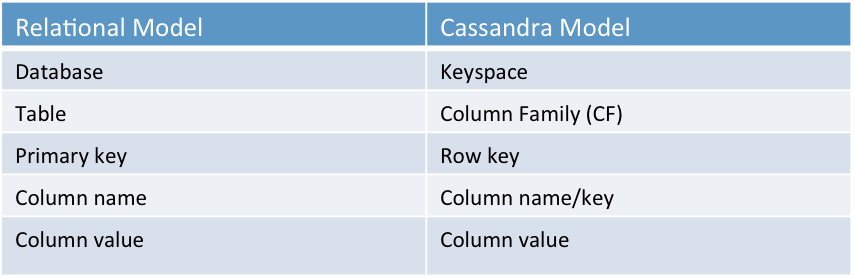
\includegraphics[scale=0.5]{analogy.png}
\caption{Cassandra vs Relační databáze}
\end{center}
\end{figure}

\begin{figure}[h]
\begin{center}
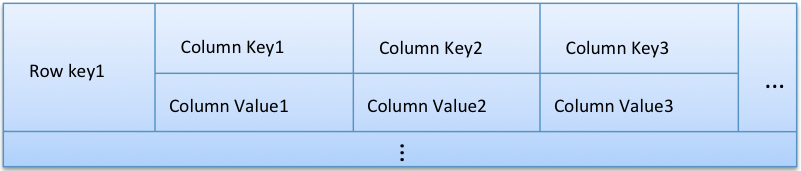
\includegraphics[scale=0.5]{RowModel.png}
\caption{Row model}
\end{center}
\end{figure}

\subsection*{Replikace}

Replikace Column Families se nastavuje na úrovni Keyspace. Z každého Row Key se vytvoří token, který určuje umístění repliky na fyzický uzel.\par

Existují různé způsoby výpočtu tokenu. Tyto způsoby jsou:

\begin{itemize}
\item \textbf{Murmur3Partitioner} - Jedná se o počáteční hodnotu, která rozmisťuje data rovnoměrně po clusteru na základě MurMur3 hashovací funkce.

\item \textbf{RandomPartitioner} -  Rovnoměrně umisťuje data po clusteru na základě MD5 hashovací funkce (je pomalejší než MurMur3).

\item \textbf{ByteOrderedPartitioner} - Ukládá data po clusteru na základě lexikálního pořadí bytů. Nedoporučuje se kvůli složitému vyvažování a nerovnoměrné distribuci dat. Jedinou výhodou je sekvenční hledání podobných klíčů.
\end{itemize}

Dále existují dva způsoby jak umísťovat další repliky. Ty jsou:

\begin{itemize}
\item \textbf{Jednoduchá strategie} - Využívá se pouze pro clustery uložené v jednom datovém centru. Tato strategie uloží první repliku na uzel určený rozdělovačem a ostatní repliky jsou uloženy na následujících uzlech v kruhu po směru hodinových ručiček bez ohledu na topologii.

\item \textbf{Síťová strategie} - Globální replikační faktor se zde změní na replikační faktor pro každé datacentrum. Každé datacentrum má vlastní kruh. Rozmisťování kopií tedy funguje následovně: První kopie se uloží na uzel vybraný rozdělovačem a další kopie ve stejném datacentru se uloží na nejbližší uzel po směru hodinových ručiček, který se nachází v jiném racku.
\end{itemize}

\section*{Modelování}

Je vhodné modelovat Cassandra databázy podle dotazů. Nelze rozšířít množství dotazů za pomoci sekundárního indexu jako u relačních databází.

\end{document}
